\documentclass[a4paper, 12pt]{article}
\newcommand{\template}{../../Templates}
\usepackage{\template/package}
\usepackage{caption}
\usepackage{tikz}
\usepackage{xcolor}
\usepackage{pgfplots}

\definecolor{colore1}{RGB}{70,188,198}
\definecolor{colore2}{RGB}{66,134,245}
\definecolor{colore3}{RGB}{234,66,53}
\definecolor{colore4}{RGB}{250,189,3}
\definecolor{colore5}{RGB}{147, 112, 219}
\definecolor{colore6}{RGB}{0,128,0}
\graphicspath{{../../Assets}}

\newcommand{\Titolo}{Piano di progetto}
\newcommand{\Data}{19/05/2024}
\newcommand{\Versione}{2.0.0}
\newcommand{\Descrizione}{Descrizione dell'organizzazione del gruppo e della pianificazione delle attività}
\newcommand{\Stato}{Approvato}
\newcommand{\Verificatori}{Alessandro Tigani Sava \\ 
& Niccolò Carlesso, Matteo Bando \\
& Giacomo Gualato, Davide Maffei}
\newcommand{\Destinatari}{prof. Tullio Vardanega \\ & prof. Riccardo Cardin}
\newcommand{\Redattori}{
    Carlo Rosso, Giacomo Gualato \\
    & Davide Maffei, Niccolò Carlesso}
\newcommand{\Approvatori}{Davide Maffei}
% Definizione dell'abbreviazione SAL
\newcommand{\SAL}{Stato di Avanzamento del Lavoro}

\newcommand{\Gruppo}{SWEnergy}
\newcommand{\Mail}{\href{mailto:project.swenergy@gmail.com}{project.swenergy@gmail.com}}
\newcommand{\g}{$^G$ }

\renewcommand\familydefault{\sfdefault} % Set default font family to sans-serif
\linespread{1.5}

\hypersetup{
	pdfmenubar=true,            % show Acrobat’s menu?
	pdfstartview={FitH},        % fits the width of the page to the window
	colorlinks=true,            % false: boxed links; true: colored links
	linkcolor=black,            % color of internal links (change box color with linkbordercolor)
	% citecolor=green,          % color of links to bibliography
	% filecolor=magenta,        % color of file links
	urlcolor=[RGB]{156,1,198}   % color of external links
}

% Define the subsubsubsection command
\newcounter{subsubsubsection}[subsubsection]
\renewcommand{\thesubsubsubsection}{\thesubsubsection.\arabic{subsubsubsection}}
\newcommand{\subsubsubsection}[1]{\refstepcounter{subsubsubsection}\subsubsection*{\thesubsubsubsection\quad#1}}

% Define the subsubsubsubsection command
\newcounter{subsubsubsubsection}[subsubsubsection]
\renewcommand{\thesubsubsubsubsection}{\thesubsubsubsection.\arabic{subsubsubsubsection}}
\newcommand{\subsubsubsubsection}[1]{\refstepcounter{subsubsubsubsection}\subsubsection*{\thesubsubsubsubsection\quad#1}}


% Define cref references
\crefname{section}{Sezione \S}{Sezioni}
\crefname{subsection}{Sottosezione \S}{Sottosezioni}
\crefname{subsubsection}{Sottosezione \S}{Sottosezioni}
\crefname{subsubsubsection}{Sottosezione \S}{Sottosezioni}
\crefname{subsubsubsubsection}{Sottosezione \S}{Sottosezioni}

\setcounter{secnumdepth}{5} % Set the section numbering depth

\newcommand{\copertina}{
	\begin{titlepage}
		\vspace*{-3.5cm}
		\makebox[\textwidth]{\includegraphics[width=\paperwidth]{header.png}}
		\begin{center}
			\includegraphics[width=1\textwidth]{logo.png}	\\
			\vspace{1cm}
			\Mail	\\
			\vspace{0.5cm}
			\textbf{\begin{LARGE} \Titolo \end{LARGE}}		\\
			\vspace{1cm}
			\textbf{Descrizione:} \Descrizione{}			\\
			\vspace{1cm}
			\begin{tabular}{ll}
				\textbf{Stato}               & \Stato              \\
				\textbf{Data}                & \Data               \\
				\midrule
				\textbf{Redattori}           & \Redattori          \\
				\textbf{Verificatori}        & \Verificatori       \\

				\ifdefined\Approvatori
				\textbf{Approvatori}         & \Approvatori        \\
				\fi

				\ifdefined\ApprovatoriInterni
				\textbf{Approvatori interni} & \ApprovatoriInterni \\
				\fi

				\ifdefined\ApprovatoriEsterni
				\textbf{Approvatori esterni} & \ApprovatoriEsterni \\
				\fi

				\ifdefined\Destinatari
				\textbf{Destinatari}         & \Destinatari        \\
				\fi

				\midrule

				\ifdefined\Versione
				\textbf{Versione}            & \Versione           \\
				\fi
			\end{tabular}
		\end{center}
		\vspace{4cm}
	\end{titlepage}
	\newpage
}

\fancypagestyle{plain}{
	\fancyhf{}
	\rhead{ \includegraphics[scale=0.05]{horizontal_logo.png}}
	\lhead{\Titolo \ifdefined\Versione \ \Versione \fi}
	%\lfoot{\Titolo}
	\rfoot{\thepage{} di \pageref{LastPage}}
	\renewcommand{\headrulewidth}{0.2pt}
	\renewcommand{\footrulewidth}{0.2pt}
}
\pagestyle{plain}

%
% RISK COMMANDS
%

%
% Rischi tecnologici
%

% Create a new counter that resets within each subsection
\newcounter{risktech}[subsection]
% Define the numbering format for the new command
\renewcommand{\therisktech}{\arabic{risktech}}

\makeatletter
\newcommand{\l@risktech}{\@dottedtocline{3}{3.8em}{3.2em}} % Formatting similar to subsubsections in TOC

% Redefine the \risktech command
\newcommand{\risktech}[1]{%
	\refstepcounter{risktech}%
	\addcontentsline{toc}{risktech}{\protect\numberline{RT-\therisktech}#1}%
	\noindent\textbf{RT-\therisktech \ #1}%
}
\newcommand{\risktechautorefname}{RT-\hspace{-0.33em}}

%
% Rischi comunicativi
%

% Idem for riskcom
\newcounter{riskcom}[subsection]
\renewcommand{\theriskcom}{\arabic{riskcom}}
\newcommand{\l@riskcom}{\@dottedtocline{3}{3.8em}{3.2em}}
\newcommand{\riskcom}[1]{%
	\refstepcounter{riskcom}%
	\addcontentsline{toc}{riskcom}{\protect\numberline{RC-\theriskcom}#1}%
	\noindent\textbf{RC-\theriskcom \ #1}%
}
\newcommand{\riskcomautorefname}{RC-\hspace{-0.33em}}

%
% Rischi organizzativi
%

% Idem for riskplan
\newcounter{riskplan}[subsection]
\renewcommand{\theriskplan}{\arabic{riskplan}}
\newcommand{\l@riskplan}{\@dottedtocline{3}{3.8em}{3.2em}}
\newcommand{\riskplan}[1]{%
	\refstepcounter{riskplan}%
	\addcontentsline{toc}{riskplan}{\protect\numberline{RP-\theriskplan}#1}%
	\noindent\textbf{RP-\theriskplan \ #1}%
}
\newcommand{\riskplanautorefname}{RP-\hspace{-0.33em}}
\makeatother

\newcounter{sprint}[section] % create a new counter for subsections

% Define the command for subsection-like elements with independent numbering
\newcommand{\sprint}[1]{%
	\stepcounter{sprint}% Increment the subsection-like counter
	\subsection*{#1~--~\arabic{sprint}}% Display subsection-like heading with custom numbering
	\addcontentsline{toc}{subsection}{\protect\numberline{\arabic{section}.\arabic{sprint}}#1}% Add to table of contents
}


\begin{document}

\copertina{}
\section*{Registro delle modifiche}
 {
  \renewcommand{\arraystretch}{1.5}
  \scriptsize
  \begin{longtable}{p{0.10\linewidth}p{0.10\linewidth}p{0.15\linewidth}p{0.15\linewidth}p{0.10\linewidth}p{0.24\linewidth}}
	  \textbf{Versione} & \textbf{Data} & \textbf{Redattore} & \textbf{Verificatore} & \textbf{Approvatore} & \textbf{Modifiche}                                 \\
	  \toprule
	  0.2.1             & 2024-05-16    & Carlo Rosso        & /
	  & /                    & Conclusione della descrizione dei pattern usati
	  nel frontend \\
	  \hline
	  0.2.0             & 2024-05-15    & Carlo Rosso        & /
	  & /                    & Ridefinizione della struttura del documento.
	  Descrizione dell'architettura di deployment e dei pattern architetturali.
	  Inizio della descrizione dei pattern usati nel frontend \\
	  \hline
	  0.1.0             & 2024-04-03    & Carlo Rosso        & /                     & /                    & Prima stesura delle sezioni 2 e 3                  \\
	  \hline
	  0.1.0             & 2024-03-30    & Carlo Rosso        & /                     & /                    & definizione della struttura generale del documento \\
	  \bottomrule
  \end{longtable}
 }

\newpage
\tableofcontents
\newpage
\section{Introduzione}
\subsection{Descrizione del documento}
Il  seguente documento ha lo scopo di indicare il \textit{way of working} del gruppo di lavoro specificando gli strumenti utilizzati e le convenzioni interne adottate.\\
\noindent
Ogni particolare termine utilizzato all'interno dei documenti viene raccolto in di un apposito documento denominato "Glossario", contenente un glossario ed un registro degli acronimi, al fine di eliminare ogni possibile ambiguità.
\section{Analisi dei rischi}

La seguente sezione ha lo scopo di identificare e catalogare i rischi che
potrebbero verificarsi durante lo svolgimento del progetto, per poterli
prevenire o almeno provare a mitigarli.
Ciascun rischio è descritto seguendo la struttura:
\begin{itemize}
	\item \textbf{Codice identificativo} seguito da un numero progressivo:
	      \begin{itemize}
		      \item \textbf{RT}: rischi legati alle tecnologie;
		      \item \textbf{RC}: rischi legati alla comunicazione;
		      \item \textbf{RP}: rischi legati alla pianificazione.
	      \end{itemize}

	\item \textbf{Titolo}: il nome che identifica il rischio;

	\item \textbf{Descrizione}: una breve descrizione del rischio;

	\item \textbf{Identificazione}: in quale modo il \textit{team} può capire se
	      si sta verificando qualche danno;

	\item \textbf{Mitigazione}: come il \textit{team} ha modo di prevenire o
	      attenuare i danni causati dal rischio;
\end{itemize}

Dopo la descrizione di ciascun rischio, viene presentata una tabella che
riassume i rischi individuati, associando a ciascuno un indice di gravità e un
indice di frequenza.

\subsection{Rischi legati alle tecnologie}
\risktech{Conoscenza delle tecnologie carente}
\label{risk:conoscenza tecnologie carente}
\begin{itemize}
	\item \textbf{Descrizione}:
		Durante lo sviluppo del progetto, potrebbe verificarsi la situazione 
		in cui almeno un membro del \textit{team} non possiede una conoscenza 
		sufficiente di una tecnologia adottata dal gruppo e necessaria per 
		lo sviluppo del progetto.

	\item \textbf{Identificazione}: 
		Il \textit{team} ha identificato le tecnologie conosciute dal gruppo 
		attraverso discussioni e accordi con il proponente. 
		Questo processo ha permesso di individuare le tecnologie non conosciute dal gruppo.

	\item \textbf{Mitigazione}:
	      \begin{itemize}
		      \item \textbf{\textit{Workshop} interni}: si rimanda alla
		            sotto-sezione "Organizzare un \textit{workshop}" del
		            documento "Norme di progetto" sotto il ruolo di progettista;

		      \item \textbf{Seminari con il proponente}: il \textit{team}
		            partecipa a seminari organizzati con il proponente, per approfondire
		            le tecnologie non conosciute. 
					Il proponente spiegherà le tecnologie e fornirà esempi di codice
		            per illustrarne l'utilizzo;

		      \item \textbf{Dialogo con il proponente}: il \textit{team} può
		            contattare il proponente per chiarimenti sulle
		            tecnologie non conosciute;

		      \item \textbf{\textit{Code review}}: si rimanda alla sotto-sezione
		            "Verifica del codice" del documento "Norme di progetto"
		            sotto il ruolo di verificatore;

		      \item \textbf{Divisione del \textit{front-end} e del \textit{back-end}}: 
			  		il \textit{team} si suddivide in due sottogruppi, uno responsabile del 
					\textit{front-end} e l'altro del \textit{back-end}. 
					Questa divisione riduce l'\textit{overhead} di comunicazione e di cambio di
		            contesto. I due gruppi si scambiano i ruoli al termine della prima 
					fase del progetto: RTB.
	      \end{itemize}
	
	\item \textbf{Riscontro}: Nessuna conseguenza significativa è stata riscontrata in quanto le misure di mitigazione necessarie sono state tempestivamente implementate
	ed i componenti del gruppo si sono riuniti al più presto per poter risolvere la problematica. Particolarmente utili si sono rilevati i \textit{workshop} interni,
	un dialogo attivo con il proponente e la divisione del \textit{team} in due sottogruppi per il \textit{front-end} e il \textit{back-end}. Mentre per quanto riguarda la mitigazione 
	prevista "Seminari con il proponente" nononostante sia stata attuata non si è rivelata del tutto efficace, per questo motivo il gruppo non ha ritenuto necessario farne uso ulteriormente.
	Una criticità riscontrata per quanto riguarda la divisione del \textit{team} in due sottogruppi sono state le difficoltà di comunicazione tra i due gruppi e formazione dei componenti, 
	che ha portato ad un rallentamento nello sviluppo del progetto.
\end{itemize}

\risktech{Strumenti \textit{software} inadeguati}
\label{risk:strumenti software inadeguati}
\begin{itemize}
	\item \textbf{Descrizione}: l'utilizzo di strumenti \textit{software} datati o poco
	      efficienti potrebbe causare ritardi nello sviluppo del progetto;

	\item \textbf{Identificazione}:
	      \begin{itemize}
		      \item Durante le riunioni interne, è cruciale prestare attenzione 
			  		ai \textit{feedback}\g dei membri del gruppo che potrebbero esprimere 
					preoccupazioni sull'efficienza o l'adeguatezza degli strumenti \textit{software} utilizzati;

		      \item I membri del gruppo potrebbero segnalare procedure troppo lunghe o 
			  		che possono essere facilmente automatizzate;

		      \item I membri del gruppo potrebbero segnalare procedure troppo lunghe o 
			  		che possono essere facilmente automatizzate. 
					Questo tipo di \textit{feedback} può indicare che gli strumenti attuali 
					potrebbero non essere ottimali per il processo di sviluppo.
	      \end{itemize}

	\item \textbf{Mitigazione}:
	      \begin{itemize}

			\item \textbf{Controllo delle Versioni da Parte dell'Amministratore}: 
				L'amministratore del progetto deve monitorare attentamente le versioni 
				degli strumenti \textit{software} utilizzati per assicurare che siano aggiornate e efficienti.
				
			\item \textbf{Informazione da parte dei membri del gruppo}: 
				I membri del gruppo devono essere proattivi nell'informarsi su nuove tecnologie e 
				strumenti \textit{software} che potrebbero migliorare l'efficienza del processo di sviluppo.

			\item \textbf{Automazione}: 
				I membri del gruppo analizzano e controllano se le procedure utilizzate siano 
				automatizzabili per migliorare l'efficienza.
	      \end{itemize}
\end{itemize}

\risktech{Codice incomprensibile}
\label{risk:codice incomprensibile}
\begin{itemize}
	\item \textbf{Descrizione}: il codice prodotto da qualche membro del gruppo
	      è di difficile comprensione per gli altri membri del gruppo.
	\item \textbf{Identificazione}:
	      \begin{itemize}
		      \item \textbf{\textit{Code review}}: durante la verifica del
		            codice, i verificatori possono riscontrare difficoltà nella
		            comprensione del codice;

	      \end{itemize}
	\item \textbf{Mitigazione}:
	      \begin{itemize}
		      \item \textbf{"Norme di progetto"}: il gruppo stila delle linee
		            guida da seguire per la stesura del codice, in modo da
		            uniformare la stesura del codice e facilitarne la
		            comprensione. Le norme sono disponibili nel documento
		            "Norme di progetto" alla sotto-sezione "Codifica" sotto il
		            ruolo di programmatore;

		      \item \textbf{\textit{Testing}}: il codice deve essere testato
		            in modo approfondito, per facilitarne la comprensione e
		            illustrarne i casi d'uso. Si rimanda alla sotto-sezione
		            "Revisione del codice" del documento "Norme di progetto"
		            sotto il ruolo di verificatore;
	      \end{itemize}
\end{itemize}


\subsection{Rischi legati alla comunicazione}
\riskcom{Comunicazione interna carente}
\label{risk:comunicazione interna carente}
\begin{itemize}
	\item \textbf{Descrizione}:
	      La comunicazione interna non è efficace ed efficiente, causando riunioni
	      interne più lunghe del previsto e rallentando le attività.
	\item \textbf{Identificazione}:
	      \begin{itemize}
		      \item \textbf{Dubbi ripetuti}: durante le riunioni interne, i
		            membri del gruppo possono porre domande già presentate in
		            precedenza;

		      \item \textbf{Riunioni interne lunghe}: le riunioni interne
		            possono protrarsi oltre il tempo previsto;

		      \item \textbf{Fraintendimenti frequenti}: i membri del gruppo
		            possono fraintendersi frequentemente.

	      \end{itemize}
	\item \textbf{Mitigazione}:
	      \begin{itemize}
		      \item \textbf{Documentazione}: il gruppo stila una documentazione
		            adeguata per facilitare la comunicazione interna. A seconda
		            dell'argomento la documentazione può avere diverse forme;

		      \item \textbf{\textit{Meeting} frequenti}: il gruppo si impegna a
		            tenere riunioni interne frequenti, in modo da ridurre la
		            durata delle riunioni interne e facilitare la comunicazione
		            interna;

		      \item \textbf{Ordine del giorno}: ciascuna riunione deve avere
		            l'ordine del
		            giorno ben definito, per discutere di tutti gli argomenti
		            utili allo sviluppo del progetto e per definire la durata di
		            ciascuno dei punti dell'ordine del giorno;

		      \item \textbf{Retrospettiva}: durante la retrospettiva, il gruppo
		            deve pensare a soluzioni \textit{ad hoc} per migliorare la
		            comunicazione interna.
	      \end{itemize}
\end{itemize}

\riskcom{Conflitti decisionali}
\label{risk:conflitti decisionali}
\begin{itemize}
	\item \textbf{Descrizione}:
	      Il gruppo potrebbe dilungarsi nella discussione di una sola idea, senza
	      raggiungere una decisione finale.
	\item \textbf{Identificazione}:
	      \begin{itemize}
		      \item un punto dell'ordine del giorno subisce un ritardo grave;
	      \end{itemize}
	\item \textbf{Mitigazione}:
	      \begin{itemize}
		      \item dibattito: i membri del gruppo discutono riguardo
		            all'importanza del punto dell'ordine del giorno, per capire se
		            è necessario approfondire la discussione o meno;

		      \item approfondimento: se il punto dell'ordine del giorno è
		            ritenuto importante, almeno due membri del gruppo si impegnano
		            a studiare i pro ed i contro delle varie soluzioni possibili.
		            Può essere chiesto un supporto al proponente oppure al
		            committente per chiarire i dubbi;

		      \item votazione: alla fine del dibattito i membri del gruppo
		            votano per la soluzione che ritengono più opportuna. La
		            votazione si ritiene conclusa quando la maggioranza dei
		            membri del gruppo ha espresso la propria preferenza e il
		            risultato non è un pareggio.

		      \item il responsabile ha il compito di vigilare sul corretto
		            svolgimento del dibattito e della votazione, in modo da
		            evitare che si dilunghi troppo.
	      \end{itemize}
\end{itemize}

\riskcom{Comunicazione esterna carente}
\label{risk:comunicazione esterna carente}
\begin{itemize}
	\item \textbf{Descrizione}:
	      Le comunicazioni con il proponente o con il committente non sono
	      efficaci ed efficienti, causando riunioni esterne più lunghe del
	      previsto e rallentando le attività; oppure rallentando le attività
	      del gruppo a causa di risposte tardive o mancanti.

	\item \textbf{Identificazione}:
	      \begin{itemize}
		      \item \textbf{Dubbi ripetuti}: durante le riunioni esterne, i
		            membri del gruppo possono porre domande già presentate in
		            precedenza;

		      \item \textbf{Riunioni esterne lunghe}: le riunioni esterne
		            possono protrarsi oltre il tempo previsto;

		      \item \textbf{Risposte tardive o mancanti}: il proponente o il
		            committente può rispondere in ritardo o non rispondere
		            affatto alle comunicazioni del gruppo.
	      \end{itemize}

	\item \textbf{Mitigazione}:
	      \begin{itemize}
		      \item \textbf{Ordine del giorno}: il responsabile si impegna a
		            stilare l'ordine del giorno delle riunioni esterne, per
		            tempo, ne discute la struttura con il gruppo e lo condivide
		            con il proponente e con il committente in anticipo;

		      \item \textbf{SAL}: il gruppo si impegna a mantenere il
		            proponente aggiornato sullo stato di avanzamento del
		            progetto, in modo da ridurre la durata delle riunioni
		            esterne e migliorare la qualità del supporto del proponente;

		      \item \textbf{Retrospettive}: sono previste delle retrospettive
		            all'interno dei SAL con il proponente, durante le quali, si
		            discute la qualità delle comunicazioni e si pensa a
		            soluzioni \textit{ad hoc} per migliorare la comunicazione
		            esterna;

		      \item \textbf{Comunicazioni frequenti}: il proponente viene tenuto
		            aggiornato frequentemente sullo stato di avanzamento del
		            progetto mediante gli appositi canali di comunicazione:
		            \textit{Telegram} e \textit{email};

		      \item \textbf{Diario di bordo}: il gruppo si impegna a tenere
		            dei diari di
		            bordo, quando richiesti dal committente, per aggiornarlo
		            sullo stato di avanzamento del progetto;

		      \item \textbf{\textit{Meeting} supplementari}: se il gruppo
		            manifesta dei dubbi o delle incertezze, può richiedere dei
		            \textit{meeting} supplementare con il proponente o con il
		            committente;

		      \item \textbf{Documentazione}: il responsabile si impegna ad
		            aggiornare la documentazione inerente agli argomenti
		            trattati durante le riunioni esterne, per dare modo ai
		            membri del gruppo di consultarla in caso di dubbi o
		            incertezze.
	      \end{itemize}
\end{itemize}


\subsection{Rischi legati alla pianificazione}
I membri del gruppo non hanno mai assunto un ruolo manageriale in
precedenza e non hanno mai lavorato in un gruppo di lavoro così
numeroso. Questo porta a problemi di gestione del tempo e delle
risorse. D'altro canto, SWEnergy si rende conto che lo scopo del
progetto è proprio quello di acquisire esperienza, anche in questi
termini. Per cui, il gruppo ha deciso di individuare alcuni
rischi legati alla pianificazione, per poterli prevenire o mitigare.

\riskplan{Organizzazione carente}
\label{risk:organizzazione carente}
\begin{itemize}
	\item \textbf{Descrizione}:
	      Il gruppo, oppure qualche membro, potrebbe non essere in grado di
	      svolgere le proprie attività, oppure potrebbe riscontrare delle
	      difficoltà a causa di una cattiva organizzazione.
	\item \textbf{Identificazione}:
	      \begin{itemize}
		      \item membri confusi: i membri del gruppo non sanno quali sono i
		            compiti a loro assegnati, oppure non sanno come svolgerli;

		      \item carenza di risorse: sono stati assegnati più incarichi di
		            quelli sostenibili con le risorse disponibili.

		      \item scadenze non aggiornate: il gruppo o qualche suo membro non
		            è in grado di rispettare le scadenze e non sono aggiornate.
		            Si tratta di un modo molto semplice, per ricadere nel
		            sintomo individuato precedentemente.
	      \end{itemize}
	\item \textbf{Mitigazione}:
	      \begin{itemize}
		      \item il responsabile mantiene aggiornate le \textit{issue}.
		            Ciascuna \textit{issue} deve essere ben documentata nella
		            propria descrizione; se è il caso, si possono aggiungere i
		            riferimenti a della documentazione supplementare. Maggiori
		            informazioni sono presenti nel documento "\textit{Way of
			            working}";

		      \item ciasun componente di SWEnergy deve aggiornare le
		            \textit{issue} a cui è assegnato, in modo da tenere il
		            responsabile e l'intera organizzazione aggiornati sullo
		            stato di avanzamento dei compiti; inoltre, deve aggiungere
		            delle \textit{issue} se ritiene che ci siano delle attività
		            da svolgere. Maggiori informazioni sono presenti nel
		            documento "\textit{Way of working}";

		      \item in caso di dubbi, i membri di SWEnergy possono rivolgersi
		            al responsabile, che si occuperà di chiarire la situazione,
		            o di indirizzare il membro verso chi può aiutarlo;

		      \item il responsabile mantiene aggiornato il \textit{project} su
		            \textit{GitHub}, in particolare per quanto riguarda
		            l'assegnamento delle \textit{issue} e delle scadenze.
		            Maggiori informazioni sono presenti nel documento
		            "\textit{Way of working}";

		      \item durante le retrospettive, il gruppo discute di eventuali
		            problemi organizzativi e cerca di trovare soluzioni per
		            migliorare la pianificazione;

		      \item dialogo con il proponente: sono chiesti consigli al
		            proponente in merito, in quanto ha più esperienza
		            nel settore e ha modo di collaborare con figure manageriali.
	      \end{itemize}
\end{itemize}

\riskplan{Comprensione dei requisiti carente}
\label{risk:comprensione dei requisiti carente}
\begin{itemize}
	\item \textbf{Descrizione}:
	      Il gruppo o qualche suo membro potrebbe non essere in grado di
	      comprendere i requisiti del progetto, oppure potrebbe riscontrare
	      delle difficoltà a causa di una cattiva comprensione dei requisiti.
	\item \textbf{Identificazione}:
	      \begin{itemize}
		      \item \textbf{Dubbi}: i membri del gruppo hanno dei dubbi in merito ai
		            requisiti;

		      \item \textbf{Dibattiti sui requisiti}: i membri del gruppo
		            discutono tra loro in merito ai requisiti;

		      \item \textbf{Discrepanza nella progettazione}: i membri del
		            gruppo progettano in modo diverso, a causa di una cattiva
		            comprensione dei requisiti.
	      \end{itemize}

	\item \textbf{Mitigazione}:
	      \begin{itemize}
		      \item \textbf{Dibattito interno}: SWEnergy si è diviso in coppie
		            per approfondire i casi d'uso e i requisiti del progetto.
		            Successivamente, si è tenuta una riunione interna in cui ciascuna coppia
		            ha esposto  le proprie considerazioni e i propri dubbi. In
		            questo modo, si è cercato di chiarire i dubbi e di
		            uniformare la comprensione dei requisiti;

		      \item \textbf{"Analisi dei requisiti"}: il metodo più formale per
		            ovviare a questa situazione risulta essere
		            l'"Analisi dei requisiti".
		            I requisiti devono essere chiari e completi. Inoltre, il documento 
					include i casi d’uso, che facilitano una migliore comprensione 
					dei requisiti concordati con il proponente;

		      \item \textbf{Dialogo con il proponente}: si instaura un dialogo attivo 
			  con il proponente per discutere dei requisiti, chiarire eventuali dubbi 
			  e definire in maggior dettaglio le funzionalità del prodotto;

		      \item \textbf{Messaggi tempestivi con il proponente}: in caso di dubbi
		            semplici e veloci da risolvere, si inviano dei messaggi al
		            proponente per ottenere una risposta tempestiva, riducendo così 
					eventuali incertezze e ritardi nella comprensione dei requisiti.
	      \end{itemize}
\end{itemize}

\riskplan{Interfacce incoerenti}
\label{risk:interfacce incoerenti}
\begin{itemize}
	\item \textbf{Descrizione}:
	      Durante la fase integrativa di più componenti, risultano delle
	      incongruenze che rendono impossibile l'integrazione.
	\item \textbf{Identificazione}:
	      \begin{itemize}
		      \item \textbf{Test di integrazione falliti}: i test di
		            integrazione falliscono a causa di incongruenze tra le
		            interfacce delle componenti;

		      \item \textbf{Discussioni interne in merito alle interfacce}: i
		            membri del gruppo discutono tra loro in merito alle
		            interfacce delle componenti, per capire come risolvere le
		            incongruenze;

		      \item \textbf{Fallimento del sistema}: l'applicativo non funziona
		            in seguito ad un'integrazione.

	      \end{itemize}
	\item \textbf{Mitigazione}:
	      \begin{itemize}
		      \item \textbf{Dialogo interno}: i membri del gruppo discutono tra loro
		            in merito alle interfacce delle componenti prima di iniziare lo 
					sviluppo delle stesse. Questo anticipato confronto aiuta a identificare 
					e risolvere potenziali incongruenze;

		      \item \textbf{Test di integrazione}: si effettuano test di integrazione 
			  		approfonditi per verificare la compatibilità tra le componenti, facilitando 
			  		l'identificazione tempestiva di eventuali problemi e garantendo 
			  		un'integrazione più efficiente;

		      \item \textbf{Documentazione}: le interfacce delle componenti sono
		            documentate in modo chiaro e completo, per evitare
		            incomprensioni ed esplicitarne la struttura e la
		            compatibilità.
	      \end{itemize}
\end{itemize}

\riskplan{Costi e tempi imprevisti}
\label{risk:costi e tempi imprevisti}
\begin{itemize}
	\item \textbf{Descrizione}:
	      Durante lo sviluppo del progetto, si può incorrere in costi o
	      rallentamenti imprevisti. Si tratta, a tutti gli effetti, di arginare
	      il danno prodotto da un rischio che si è verificato.
	\item \textbf{Identificazione}:
	      \begin{itemize}
		      \item \textbf{Monitoraggio costante}: si effettua un monitoraggio 
			  		continuo dei costi e delle tempistiche al raggiungimento delle 
					\textit{milestone} e durante gli \textit{stand-up}.
			  
	      \end{itemize}
	\item \textbf{Mitigazione}:
	      \begin{itemize}
		      \item \textbf{\textit{Buffer} di tempo}: Il team ha proattivamente 
			  		inserito margini temporali tra le diverse attività, creando 
					\textit{buffer} di tempo che consentono di gestire eventuali 
					ritardi senza compromettere la pianificazione principale;

		      \item \textbf{\textit{Buffer} di costi}: il \textit{team} ha 
			  		preventivamente allocato risorse finanziarie extra, 
					sotto forma di \textit{buffer} di costi, per far fronte 
					a spese impreviste e mantenere il controllo del budget;

		      \item \textbf{Pianificazione in itinere}: il \textit{team} si adatta
		            alle variazioni dei costi e delle tempistiche di
		            completamento, per poter gestire eventuali costi
		            imprevisti. In questo caso, sono aggiornate le scadenze
		            nel \textit{project} su \textit{GitHub} e i costi.
		            A seconda della situazione, le \textit{issue} sono
		            riassegnate e le \textit{milestone} sono adattate allo
		            \textit{status quo}.
	      \end{itemize}
\end{itemize}


\subsection{Pericolosità e occorrenze}

Per ogni rischio, il \textit{team} ha individuato un indice di gravità e un
indice di frequenza, per poter stimare il rischio residuo. L'indice di
gravità e quello di frequenza sono due numeri compresi tra 1 e 5. L'indice di
rischio residuo è il prodotto tra i due indici, può quindi assumere valori
compresi tra 1 e 25. Più il rischio residuo è alto, maggiori sono i danni che
può causare e più è probabile che si verifichi. Si noti che non è detto che il
verificarsi del rischio causi i danni massimi, le strategie di
mitigazione servono proprio per prevenire e attenuare i danni.

\begin{table}[H]
	\centering

	\begin{tabular}{l|r|r|r}
		\hline
		\textbf{Rischi tecnologici}                                                          & \textbf{Gravità} & \textbf{Frequenza} & \textbf{Rischio residuo} \\
		\hline
		\autoref{risk:conoscenza tecnologie carente} Conoscenza delle tecnologie carente     & 5                & 4                  & 20                       \\
		\autoref{risk:strumenti software inadeguati} Strumenti \textit{software} inadeguati           & 1                & 2                  & 2                        \\
		\autoref{risk:codice incomprensibile} Codice incomprensibile                         & 2                & 2                  & 4                        \\
		\autoref{risk:incompatibilità delle versioni del software} 
		Incompatibilità delle versioni del \textit{software}											 & 3                & 1                  & 3                        \\
		\autoref{risk:scarsa documentazione delle tecnologie utilizzate} 
		Scarsa documentazione delle tecnologie utilizzate	   								 & 2                & 2                  & 4                        \\
		\autoref{risk:problemi di sicurezza delle tecnologie utilizzate} 
		Problemi di sicurezza delle tecnologie utilizzate	   								 & 5                & 2                  & 10                        \\
		\hline
		\multicolumn{4}{l}{}                                                                                                                                    \\
		\hline
		\textbf{Rischi comunicativi}                                                         & \textbf{Gravità} & \textbf{Frequenza} & \textbf{Rischio residuo} \\
		\hline
		\autoref{risk:comunicazione interna carente} Comunicazione interna carente           & 3                & 3                  & 9                        \\
		\autoref{risk:conflitti decisionali} Conflitti decisionali                           & 1                & 2                  & 2                        \\
		\autoref{risk:comunicazione esterna carente} Comunicazine esterna carente            & 2                & 2                  & 4                        \\
		\autoref{risk:mancanza di chiarezza nei ruoli e responsabilità}
		Mancanza di chiarezza nei ruoli e responsabilità									 & 4                & 3                  & 12                        \\
		\autoref{risk:comunicazione asincrona inefficace}
		Comunicazione asincrona inefficace									 				 & 2                & 3                  & 6                        \\
		\hline
		\multicolumn{4}{l}{}                                                                                                                                    \\
		\hline
		\textbf{Rischi organizzativi}                                                        & \textbf{Gravità} & \textbf{Frequenza} & \textbf{Rischio residuo} \\
		\hline
		\autoref{risk:organizzazione carente} Organizzazione carente                         & 3                & 4                  & 12                       \\
		\autoref{risk:comprensione dei requisiti carente} Comprensione dei requisiti carente & 2                & 3                  & 6                        \\
		\autoref{risk:interfacce incoerenti} Interfacce incoerenti                           & 4                & 2                  & 8                        \\
		\autoref{risk:costi e tempi imprevisti} Costi e tempi imprevisti                     & 5                & 3                  & 15                       \\
		\autoref{risk:cambiamenti nei requisiti} Cambiamenti nei requisiti                   & 5                & 1                  & 5                        \\
		\hline
	\end{tabular}
	\caption{Tabella della pericolosità e dell'occorrenza dei rischi.}
\end{table}


\section{Modello di sviluppo}

\subsection{Modello incrementale}
SWEnergy ha deciso di adottare il modello di sviluppo incrementale, che prevede
la suddivisione del progetto in incrementi. Al completamento di ciascun
incremento viene rilasciata una nuova versione del prodotto, che è mostrata al
proponente durante le riunioni di revisione. Poiché il \textit{team} non ha mai
lavorato in ambito professionale, il modello di sviluppo è ispirato al
\textit{framework} Scrum con \textit{sprint} di due settimane, con qualche
modifica per adattarlo alle esigenze del progetto e del gruppo. In particolare,
SWEnergy introduce una retrospettiva \textit{in media res} per valutare il
lavoro svolto e apportare eventuali modifiche al processo di sviluppo.
In aggiunta, non sono previste le \textit{daily stand-up meeting}, in quanto il
gruppo ritiene che la cadenza delle suddette sia troppo elevata considerando
che il progetto è svolto da studenti universitari e non da lavoratori a tempo
pieno.

\subsection{Iterazioni}

\subsubsection{\textit{Sprint}}
Uno \textit{sprint} ha una durata di due settimane. Durante questo periodo, il
gruppo si impegna a sviluppare l'incremento del prodotto concordato con il
proponente. La durata di uno \textit{sprint} è stata scelta sulle esigenze del
proponente;
permette al \textit{team} di effettuare un mini-\textit{sprint} di una
settimana; consente di ricevere \textit{feedback} frequenti dal proponente e di
apportare modifiche al prodotto in modo tempestivo. In aggiunta, permette al
\textit{team} di risolvere eventuali problemi o dubbi con il proponente in modo
dinamico, flessibile e tempestivo. I mini-\textit{sprint} aumentano la frequenza
delle retrospettive e mantengono il gruppo focalizzato sul lavoro da svolgere.
Permettono di valutare lo svolgimento delle attività durante lo \textit{sprint}
e di apportare modifiche al processo di sviluppo adattando il lavoro alle
esigenze del progetto.

\subsubsection{Mini-\textit{sprint}}
Questa iterazione emula il \textit{framework} Scrum, con una cadenza settimanale
piuttosto che bisettimanale o mensile. Si tratta di uno \textit{sprint}
interno al gruppo: il proponente non viene coinvolto. Al termine di un
mini-\textit{sprint} potrebbe corrispondere un cambio dei ruoli, in base alle
esigenze del progetto e del gruppo.

\subsection{Eventi}

\subsubsection{SAL}
Lo Stato di Avanzamento del Lavoro (SAL) è un incontro con il proponente che
avviene ogni due settimane di venerdì. Queste riunioni sono utili per
condividere i \textit{feedback} in entrambe le direzioni: il proponente può
valutare il lavoro svolto dal gruppo; e SWEnergy può esprimere le proprie
opinioni sul prodotto. Di seguito sono riportate le attività principali che
avvengono durante un SAL:

\begin{itemize}
	\item \textbf{\textit{Sprint review}}: Il gruppo presenta il lavoro svolto
	      durante lo
	      \textit{sprint} e il proponente fornisce dei \textit{feedback} sul
	      prodotto. In aggiunta, il gruppo può porre domande per chiarire
	      eventuali dubbi in merito ai requisiti e alle funzionalità richieste,
	      oppure in merito all'implementazione di queste ultime.

	\item \textbf{\textit{Sprint retrospective}}: Il gruppo discute sulle modalità
	      di lavoro. In particolare, valuta se il processo di sviluppo
	      è stato efficace ed efficiente ed in quale modo sia migliorabile.
	      Sono chiesti consigli al proponente in merito all'organizzazione del
	      lavoro; sono riportati eventuali problemi riscontrati durante lo
	      \textit{sprint} e sono proposte soluzioni per risolverli.

	\item \textbf{\textit{Sprint planning}}: Il gruppo e il proponente concordano
	      l'incremento del prodotto da sviluppare durante lo \textit{sprint}
	      successivo; ovvero che cosa inserire nello \textit{sprint backlog}.
\end{itemize}

\subsubsection{\textit{Stand-up}}
Il nome \textit{stand-up} è ispirato ai \textit{daily stand-up meeting} del
\textit{framework} Scrum. Si noti che l'incontro con il proponente avviene un
venerdì su due; mentre le \textit{stand-up}, gli incontri all'inizio
e al termine di un mini-\textit{sprint}, hanno luogo ogni domenica,
per dare modo al responsabile di considerare i \textit{feedback} del proponente
e di pianificare l'iterazione successiva. L'organizzazione viene poi discussa
durante la \textit{stand-up}. Di seguito sono riportate le attività principali
che avvengono durante una \textit{stand-up}:

\begin{itemize}
	\item \textbf{\textit{Brainstorming}}: Il responsabile riassume il lavoro
	      svolto durante la settimana e ciascun membro del gruppo può arricchire
	      la spiegazione con le proprie esperienze, per esempio, descrivendo le
	      difficoltà incontrate e le soluzioni adottate.

	\item \textbf{Retrospettiva}: Il gruppo discute sulle modalità di
	      lavoro. In particolare, valuta se il processo di sviluppo è stato
	      efficace ed efficiente ed in quale modo sia migliorabile. Sono
	      riportati eventuali problemi riscontrati durante il
	      mini-\textit{sprint} e sono proposte soluzioni per risolverli.
	      Eventualmente si prende nota dei problemi per discuterne con il
	      proponente durante il SAL; oppure per domandare consigli al
	      committente.

	\item \textbf{Pianificazione}: Il responsabile mostra la pianificazione del
	      mini-\textit{sprint} successivo. I membri del gruppo possono
	      intervenire per proporre miglioramenti o per chiarire eventuali dubbi.
	      Infine, il responsabile assegna i compiti ai membri del gruppo,
	      secondo le loro disponibilità, capacità e preferenze.
\end{itemize}

Risulta utile dividere le \textit{stand-up} in due gruppi: le \textit{stand-up}
che avvengono la domenica successiva al SAL sono dedicate alla pianificazione
del mini-\textit{sprint} successivo; mentre le \textit{stand-up} che avvengono
la domenica successiva sono principalemente dedicate alla retrospettiva del
mini-\textit{sprint} appena concluso. Queste ultime sono utilizzate anche per
organizzare il SAL successivo: il responsabile raccoglie i problemi riscontrati;
organizza le domande da porre al proponente; e pianifica l'ordine del giorno del
SAL. Il \textit{team} può richiedere qualche modifica all'ordine del giorno. In
questo modo, è possibile anticipare eventuali problemi e risolverli prima del
SAL, evitando di sprecare tempo prezioso. In aggiunta, il responsabile può
condividere l'ordine del giorno con il proponente prima del SAL. Si noti
che è prevista una vera e propria \textit{stand-up}, della durata di circa 30
minuti, anche tra il giovedì o il venerdì precedente al SAL, per effetturare un
veloce \textit{brainsorming}, raccogliere le ultime domande e modificare
l'ordine del giorno in base alle risposte del proponente e alle necessità del
gruppo.

\subsection{Motivazioni}

SWEnergy ha deciso di organizzarsi come descritto in precedenza più per
necessità che per scelta: durante i corsi di Ingegneria del Software e di Metodi
e Tecnologie per lo Sviluppo Software, i membri del gruppo hanno appreso i
concetti fondamentali del \textit{framework} Scrum. Dunque, il \textit{team} ha
deciso di metterli in pratica. Come già accennato, il gruppo non ha mai lavorato
in un ambito professionale e non ha esperienza con i metodi di lavoro ed
organizzativi. In aggiunta, il proponente ha richiesto una pianificazione di
almeno due settimane.
Con la seguente organizzazione, SWEnergy spera di riuscire a soddisfare le
esigenze del proponente mitigando i rischi individuati durante l'analisi dei
rischi. Il \textit{framework} Scrum dovrebbe fornire i seguenti vantaggi:

\begin{enumerate}
	\item \textbf{Flessibilità}: Il gruppo può adattare il processo di sviluppo
	      alle esigenze del progetto. In particolare, il gruppo
	      può modificare la pianificazione in base alle esigenze del
	      proponente e del gruppo.

	\item \textbf{Comunicazione trasparente}: Il gruppo può rilasciare
	      incrementi del prodotto in modo tempestivo. In aggiunta, il
	      proponente può valutare il lavoro svolto dal gruppo e fornire
	      \textit{feedback} in itinere, approfondendo i requisiti.

	\item \textbf{Miglioramento continuo}: Le retrospettive permettono al
	      gruppo di valutare il processo di sviluppo e di apportare
	      modifiche per migliorarlo. In aggiunta, il gruppo può
	      discutere con il proponente o con il committente per ricevere consigli
	      e suggerimenti per migliorare l'organizzazione.

	\item \textbf{Monitoraggio costante}: La pianificazione basata sugli
	      \textit{sprint} permette di identificare e affrontare rischi in modo
	      più tempestivo, riducendo la possibilità di ritardi gravi.
\end{enumerate}

\section{Pianificazione}

\subsection{RTB}

\subsubsection{Prima fase}

\subsubsection{Stesura delle bozze}

\subsubsection{Progettazione e prototipazione}

\subsubsection{Stesura della documentazione}

\subsubsection{Creazione del \gls{POC}$^G$}

\subsubsection{Retifica della documentazione}

\subsection{PB}

\subsection{CA}

\section{Consuntivo a finire}

Nella seguente sezione sono riportati i dati in forma tabellare 
delle ore totali preventivate per la fase RTB rispetto alle ore effettive 
utilizzate dal gruppo SWEnergy.

\subsection{Analisi RTB}



\subsubsection{Riepilogo preventivo per la fase RTB}

\begin{table}[H]
	\centering
	\begin{tabular}{l|c|c|c|c|c|c|c}
		\textbf{Nome}         & \textbf{Re} & \textbf{Am} & \textbf{An} & \textbf{Pt} & \textbf{Pr} & \textbf{Ve} & \textbf{Totale ore} \\
		\hline
		Alessandro            & 5           & -           & 5           & 15           & 10           & -           & 35              \\
		Carlo                 & 5           & 5           & 10           & 10           & 5           & -           & 35              \\
		Davide                & 5           & -           & 20          & -           & 5           & 5           & 35              \\
		Giacomo               & 5           & -           & 15          & -           & -           & 5           & 25              \\
		Matteo                & -           & 5           & 10          & -           & 10           & 10           & 35              \\
		Niccolò               & 5           & -           & 10          & 10           & -           & 10           & 35              \\
		\hline
		%\textbf{Ore totali}   & 25          & 10           & 70          & 35           & 30           & 30           & 60              \\
		%\textbf{Costo totale} & 300         & 100         & 1000        & 125         & -           & -           & 1525
	\end{tabular}
	\caption{Re: Responsabile, Am: Amministratore, An: Analista, Pt: Progettista,
		Pr: Programmatore, Ve: Verificatore, Totale: Totale per persona; valori espressi in ore; Costo totale espresso in euro.}
\end{table}




\subsubsection{Riepilogo consuntivo per la fase RTB}

\begin{table}[H]
	\centering
	\begin{tabular}{l|c|c|c|c|c|c|c}
		\textbf{Nome}         & \textbf{Re} & \textbf{Am} & \textbf{An} & \textbf{Pt} & \textbf{Pr} & \textbf{Ve} & \textbf{Totale ore} \\
		\hline
		Alessandro            & 5           & 5           & 5           & 10           & 10           & -           & 35              \\
		Carlo                 & 10           & 10           & 10           & -           & 5           & -           & 35              \\
		Davide                & 5           & -           & 20          & -           & 5           & 5           & 35              \\
		Giacomo               & 5           & 5           & 5          & 10           & -           & 10           & 35              \\
		Matteo                & -           & 5           & 10          & 5           & 10           & 5           & 35              \\
		Niccolò               & 5           & -           & 10          & 10           & -           & 10           & 35              \\
		\hline
		%\textbf{Ore totali}   & 30          & 25           & 60          & 35          & 30           & 30           & 60              \\
		%\textbf{Costo totale} & 300         & 100         & 750         & 375         & -           & -           & 1525
	\end{tabular}
	\caption{Re: Responsabile, Am: Amministratore, An: Analista, Pt: Progettista,
		Pr: Programmatore, Ve: Verificatore, Totale: Totale per persona; valori espressi in ore; Costo totale espresso in euro.}
\end{table}






\subsubsection{Riepilogo finale RTB}

Di seguito vengono indicate le spese effettive nelle fase RTB del progetto.

\begin{table}[H]
	\centering
	\begin{tabular}{l|c|c|c|c|c|c|c}
		\textbf{Ruolo}         & \textbf{Ore P} & \textbf{Ore E} & \textbf{Diff. ore} & \textbf{Costo orario} & \textbf{Costo P} &\textbf{Costo E} & \textbf{Diff. costo}  \\
		\hline
		Responsabile            & 25                     & 30             & +5                    & 30                   & 750           & 900                     & +150              \\
		Amministratore          & 10                     & 25             & +15                   & 20                   & 200           & 500                     & +300              \\
		Analista                & 70                     & 60             & -10                   & 25                   & 1750           & 1500                   & -250              \\
		Progettista             & 35                     & 35             & 0                     & 25                   & 875           & 875                     & 0              \\
		Programmatore           & 30                     & 30             & 0                     & 15                   & 450           & 450                     & 0              \\
		Verificatore            & 30                     & 30             & 0                     & 15                   & 450           & 450                     & 0              \\
        \hline
        Totale Consuntivo       & 200                    & 210            & +10                   &                      & 4475          & 4675                    & +200              \\
		\hline
		%\textbf{Ore totali}   & 10          & 5           & 30          & 15          & -           & -           & 60              \\
		%\textbf{Costo totale} & 300         & 100         & 750         & 375         & -           & -           & 1525
	\end{tabular}
	\caption{Consuntivo periodo RTB, Ore P: Totale Ore preventivate per un singolo ruolo, Ore e: Totale Ore effettive per un singolo ruolo, 
            Diff. ore: Differenza tra ore preventivate e ore effettive, Costo orario: costo orario di un singolo ruolo, Costo P: totale costo preventivato per un singolo ruolo, 
            Costo E: totale costo effettivo per un singolo ruolo,  Diff. costo: Differenza tra costo preventivato e costo effettivo;
            Costo orario: espresso in (\euro/h), Costo P, Costo E, Diff. costo: espressi in (\euro)}  
\end{table}






\subsubsection{Riepilogo ripartizione percentuale oraria}

\begin{figure}[h]
	\centering
	\begin{tikzpicture}
		\pie[text=legend]{
			14/Responsabile,
			12/Amministratore,
			29/Analista,
			17/Progettista,
			14/Programmatore,
			14/Verificatore
		}
	\end{tikzpicture}
	\caption{Riepilogo ripartizione percentuale oraria}
\end{figure}



\subsubsection{Suddivisione ruoli per persona}

\begin{flushleft}
    \begin{figure}[h]
        \centering
        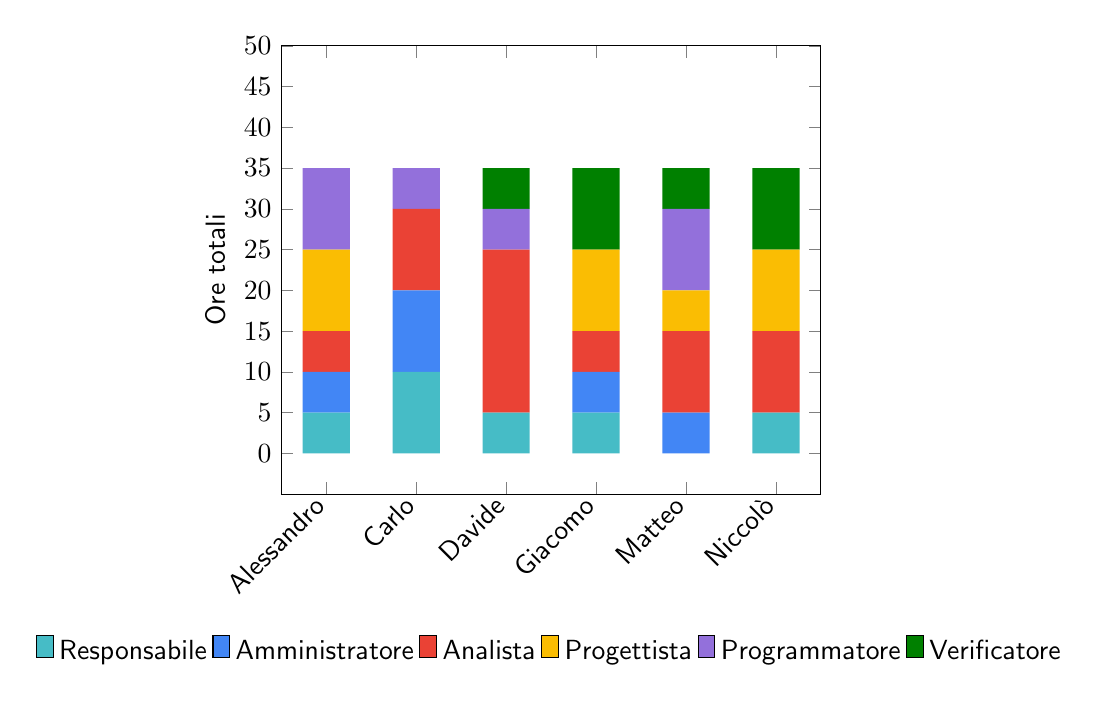
\begin{tikzpicture}
            \begin{axis}[
                ybar stacked,
                bar width=0.6cm,
                xlabel={}, % Rimuovo l'etichetta dell'asse x
                ylabel={Ore totali},
                symbolic x coords={Alessandro, Carlo, Davide, Giacomo, Matteo, Niccolò},
                xtick=data,
                x tick label style={rotate=45,anchor=east}, % Nomi obliqui di 45 gradi
                ytick={0,5,...,50}, % Suddivisione asse y ogni 5 da 0 a 50
                nodes near coords={},
                nodes near coords align={vertical},
                legend style={at={(0.5,-0.3)},anchor=north,legend columns=-1,draw=none}, % Maggiore distanza verticale
                every node near coord/.append style={font=\tiny}, % Dimensione del font delle etichette (vuoto per rimuoverle)
                every axis plot/.append style={draw=none}, % Rimuovo i bordi delle barre
                ymax=50, % Estendo l'asse y fino al valore 50
            ]
            
            % Dati per l'asse delle x
            \addplot[fill=colore1] coordinates {(Alessandro, 5) (Carlo, 10) (Davide, 5) (Giacomo, 5) (Matteo, 0) (Niccolò, 5)};
            \addplot[fill=colore2] coordinates {(Alessandro, 5) (Carlo, 10) (Davide, 0) (Giacomo, 5) (Matteo, 5) (Niccolò, 0)};
            \addplot[fill=colore3] coordinates {(Alessandro, 5) (Carlo, 10) (Davide, 20) (Giacomo, 5) (Matteo, 10) (Niccolò, 10)};
            \addplot[fill=colore4] coordinates {(Alessandro, 10) (Carlo, 0) (Davide, 0) (Giacomo, 10) (Matteo, 5) (Niccolò, 10)};
            \addplot[fill=colore5] coordinates {(Alessandro, 10) (Carlo, 5) (Davide, 5) (Giacomo, 0) (Matteo, 10) (Niccolò, 0)};
			\addplot[fill=colore6] coordinates {(Alessandro, 0) (Carlo, 0) (Davide, 5) (Giacomo, 10) (Matteo, 5) (Niccolò, 10)};
            
            \legend{Responsabile, Amministratore, Analista, Progettista, Programmatore, Verificatore}
            
            \end{axis}
        \end{tikzpicture}
        \caption*{Rappresentazione ore assegnate ad una persona che ha eseguito un determinato ruolo}
    \end{figure}
\end{flushleft}





\subsection{Considerazioni}
Prima di iniziare con le considerazioni riporto la tabella delle assegnazione 
delle ore che il gruppo SWEnergy si impegna a rispettare.

\begin{table}[H]
	\renewcommand{\arraystretch}{1.5}
	\centering
	\begin{tabular}{l|r|r|r|r|r|r|r}
		\textbf{Membro} & \textbf{Re} & \textbf{Am} & \textbf{An} & \textbf{Pt}
		& \textbf{Pr} & \textbf{Ve} & \textbf{Tot} \\
		\hline
		Alessandro Tigani Sava 	&	16 &  7 & 12 & 15 &  27 &  17 &  94 \\
		Carlo Rosso 			&	16 &  7 & 13 & 15 &  26 &  17 &  94 \\
		Davide Maffei			&	16 &  7 & 13 & 14 &  27 &  17 &  94 \\
		Giacomo Gualato 		&	16 &  8 & 12 & 15 &  26 &  17 &  94 \\
		Matteo Bando 			&	15 &  8 & 13 & 15 &  27 &  16 &  94	\\
		Niccolò Carlesso 		&	16 &  8 & 12 & 15 &  27 &  16 &  94 \\
		\hline
		\textbf{Totale} 		&	95 & 45 & 75 & 89 & 160 & 100 & 564 \\
	\end{tabular}

	\caption{Assegnamento delle ore per persona; valori espressi in ore.
		Re: Responsabile, Am: Amministratore, An: Analista, Pt:
	Progettista, Pr: Programmatore, Ve: Verificatore, Tot: Totale ore per 
	membro; valori espressi in ore.}
\end{table}

Da come si può notare, il gruppo SWEnergy ha deciso di utilizzare sulle circa 
94 ore a testa. Da come si può notare dalla sezione sopra, ciascuna persona dopo 
questi 5 \textit{sprint} è arrivata a 35 ore, quindi una rimanenza di 59 ore per la fase PB e CA.


\begin{table}[H]
	\centering
	\begin{tabular}{l|c}
		\textbf{Ruolo}         & \textbf{Ore utilizzate} \\
		\hline
		Responsabile            & 30            \\
		Amministratore          & 25            \\
		Analista                & 60            \\
		Progettista             & 35            \\
		Programmatore           & 30            \\
		Verificatore            & 30            \\
		\hline
	\end{tabular}
	\caption{Ore utilizzate per ruolo; valori espressi in ore.}  
\end{table}

Da come si può notare, il gruppo SWEnergy ha utilizzato 210 ore, quindi una rimanenza di 354 ore per la fase PB e CA.
Inoltre, rispetto a quanto preventivato si è sottostima, anche se di poco le ore del Responsabile dando meno importanza 
all'amministratore, mentre per gli altri ruoli, la suddivisione oraria pensata e preventivata all'inizio sono state ben 
ragionate e si adotteranno.
Quindi si andranno ad utilizzare circa sulle 13 ore a testa per il ruolo di Responsabile e sulle 10 ore a testa per il ruolo di Amministratore.
Inoltre, avevamo soprastimato di poco il ruolo di analista, ma lasciamo qualche ora residua per eventuali modifiche o aggiunte ai requisiti, anche se 
andiamo a ridurre quelle residue per aumentare il numero delle ore di altri ruolo più carenti.

Ecco una tabella con la nuova ripartizione oraria per la prossima fase PB:

\begin{table}[H]
	\renewcommand{\arraystretch}{1.5}
	\centering
	\begin{tabular}{l|r|r|r|r|r|r|r}
		\textbf{Membro} & \textbf{Re} & \textbf{Am} & \textbf{An} & \textbf{Pt}
		& \textbf{Pr} & \textbf{Ve} & \textbf{Tot} \\
		\hline
		Alessandro Tigani Sava 	&	8 	&  5 	& 4 	& 8 	&  17 	&  17 	&  59 \\
		Carlo Rosso 			&	5 	&  0 	& 3 	& 15 	&  21 	&  15 	&  59 \\
		Davide Maffei			&	8 	&  11 	& 0 	& 12 	&  18 	&  10 	&  59 \\
		Giacomo Gualato 		&	8 	&  7 	& 2 	& 9 	&  26 	&  7 	&  59 \\
		Matteo Bando 			&	13 	&  5 	& 3 	& 10 	&  17 	&  11 	&  59	\\
		Niccolò Carlesso 		&	8 	&  10 	& 2 	& 5 	&  27 	&  7 	&  59 \\
		\hline
		\textbf{Totale} 		&	95 & 45 & 75 & 89 & 160 & 100 & 564 \\
	\end{tabular}

	\caption{Preventivo e assegnazione ore per la fase PB; valori espressi in ore.
		Re: Responsabile, Am: Amministratore, An: Analista, Pt:
	Progettista, Pr: Programmatore, Ve: Verificatore, Tot: Totale ore per 
	membro; valori espressi in ore.}
\end{table}



\begin{table}[H]
	\centering
	\begin{tabular}{l|c|c}
		\textbf{Ruolo}         & \textbf{Ore utilizzate} 	& \textbf{Costo}\\
		\hline
		Responsabile            & 50                 & 1500     \\
		Amministratore          & 38                 & 760    \\
		Analista                & 14                 & 350     \\
		Progettista             & 59                 & 1475      \\
		Programmatore           & 126                & 1890      \\
		Verificatore            & 66                 & 990     \\
		\hline
		Costo totale			&                	 & 6965     \\
	\end{tabular}
	\caption{Suddivisione oraria per ruolo per la fase PB}  
\end{table}

Quindi se si somma il costo totale della fase RTB (4675 \euro) con il costo totale preventivato della fase PB (6965 \euro) si ottiene 
un costo totale di 11160 euro, perfettamente in linea con il budget preventivato all'inizio di 11750 \euro.


Il conclusione il gruppo SWEnergy conferma nuovamente il budget iniziale stimato e anche la data di consegna prevista al 10/05/2024




%\input{sec/chiusura.tex}
\end{document}
